\documentclass[a4paper,11pt]{ltjsarticle}
\usepackage[haranoaji]{luatexja-preset}
\usepackage{amsmath,amssymb}
\usepackage[top=12mm,bottom=10mm,left=14mm,right=14mm]{geometry}
\usepackage{array}
\usepackage{tikz}
\usetikzlibrary{calc}
\pagestyle{empty}
\setlength{\parindent}{0pt}
\newlength{\qcol}\setlength{\qcol}{0.47\textwidth}
\newlength{\qgap}
\newlength{\anscolw}\setlength{\anscolw}{0.30\textwidth}
\newlength{\ansh}
\newcommand{\Q}[2]{\parbox[t]{\qcol}{\raggedright (#1)\hspace{0.6em}$\displaystyle #2$}}
\newcommand{\QR}[4]{\Q{#1}{#2}\hfill\Q{#3}{#4}\par\vspace{\qgap}}
\newcommand{\anscell}[1]{\rule[-\ansdrop]{0pt}{\ansh}(#1)}
\newlength{\ansdrop}

\begin{document}
{\large\bfseries 数学テスト　4}\hfill 名前(\underline{\hspace{32mm}})\par\vspace{3mm}
■（1）〜（12）の計算をしなさい。（13）、（14）は連立方程式を解きなさい。\par\vspace{3mm}
\setlength{\qgap}{11mm}
\QR{1}{\dfrac{a-b}{3}-\dfrac{a+b}{4}}{2}{a-\{5b+(4a+3b)-2\}}
\QR{3}{(30x-25y)\div5}{4}{18ab^2\div3ab\times2a}
\QR{5}{(2x-3y)+(-3x+2y)}{6}{(4a^2+3a-2)-(-a^2+3a+5)}
\QR{7}{2a\times(-5ab)}{8}{2(x-y)+3(x-2y)}
\QR{9}{18a^2b\div8ab}{10}{(x+3y)+(4x-6y)-(2x+5y)}
\QR{11}{(-5x)^2}{12}{\dfrac{1}{4}(12x+16y)}
\QR{13}{\left\{\begin{array}{l} x+4y=-2 \\ 3x-4y=10 \end{array}\right.}{14}{\left\{\begin{array}{l} 3x-y=2 \\ y=-2x+3 \end{array}\right.}
\vspace{2mm}
\setlength{\ansh}{11mm}\setlength{\ansdrop}{7mm}%
\begin{center}\begin{tabular}{|p{\anscolw}|p{\anscolw}|p{\anscolw}|}\hline
\anscell{1} & \anscell{2} & \anscell{3} \\\hline
\anscell{4} & \anscell{5} & \anscell{6} \\\hline
\anscell{7} & \anscell{8} & \anscell{9} \\\hline
\anscell{10} & \anscell{11} & \anscell{12} \\\hline
\anscell{13} & \anscell{14} &  \\\hline
\end{tabular}\end{center}

\newpage

■次の図形を直線 $\ell$ を軸に1回転させてできる立体の体積と表面積を求めなさい。
\par\vspace{4mm}
\begin{minipage}[t]{0.48\textwidth}
①\par\vspace{2mm}
\hspace*{10mm}
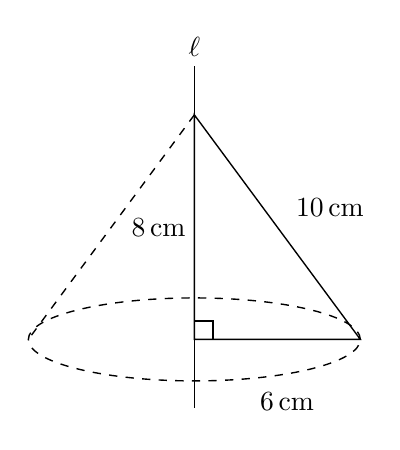
\begin{tikzpicture}[scale=0.62,line width=0.5pt]
  \draw (0,-1.4) -- (0,5.6); \node[above] at (0,5.6) {$\ell$};
  \draw[dashed] (0,0) ellipse (3.4 and 0.85);
  \draw[dashed] (0,4.6) -- (-3.4,0);
  \draw (0,4.6) -- (0,0) -- (3.4,0) -- cycle;
  \draw (0,0.38) -- (0.38,0.38) -- (0.38,0);
  \node[left,inner sep=3pt] at (0,2.3) {8\,cm};
  \node[below,inner sep=4pt] at (1.9,-0.85) {6\,cm};
  \node[right,inner sep=3pt] at (1.9,2.7) {10\,cm};
\end{tikzpicture}

\par\vspace{6mm}
\hspace*{6mm}体積(\underline{\hspace{30mm}})\par\vspace{5mm}
\hspace*{4mm}表面積(\underline{\hspace{30mm}})
\end{minipage}\hfill
\begin{minipage}[t]{0.48\textwidth}
②\par\vspace{2mm}
\hspace*{10mm}
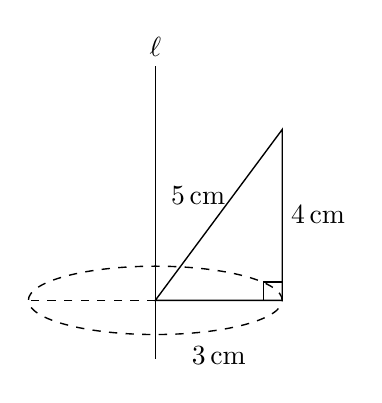
\begin{tikzpicture}[scale=0.62,line width=0.5pt]
  \draw (0,-1.2) -- (0,4.8); \node[above] at (0,4.8) {$\ell$};
  \draw[dashed] (0,0) ellipse (2.6 and 0.7);
  \draw[dashed] (0,0) -- (-2.6,0);
  \draw (0,0) -- (2.6,0) -- (2.6,3.5) -- cycle;
  \draw (2.22,0) -- (2.22,0.38) -- (2.6,0.38);
  \node[right,inner sep=3pt] at (2.6,1.75) {4\,cm};
  \node[below,inner sep=4pt] at (1.3,-0.7) {3\,cm};
  \node[above left,inner sep=1pt] at (1.5,1.9) {5\,cm};
\end{tikzpicture}

\par\vspace{6mm}
\hspace*{6mm}体積(\underline{\hspace{30mm}})\par\vspace{5mm}
\hspace*{4mm}表面積(\underline{\hspace{30mm}})
\end{minipage}

\end{document}
